\section{Numerical Results}
\label{sec:numerical_results}
To verify the performance of the proposed method we test it on two different 3D problems: a cantilever beam and the Stanford bunny. Both geometries use material properties designed to mimic soft tissue behavior, with Young's modulus $E = 10^6$ Pa and Poisson's ratio $\nu = 0.45$.

\subsubsection{Cantilever beam}
\label{sec:cantilever_beam_setup}
The first test case is a cantilever beam with a square cross-section of size $1 \times 1$ and a length of $10$. The beam is clamped at one end and free at the other. This geometry represents a classical benchmark problem in structural mechanics, allowing for clear interpretation of the modal behavior and providing a controlled environment to validate the fundamental capabilities of our neural network approach. The cantilever beam exhibits well-understood physics with distinct modal patterns: bending modes in two perpendicular directions, torsional modes, and higher-order coupled deformation modes. The soft tissue material properties result in large deformations under relatively small loads, making this an ideal test case for nonlinear mechanics validation.

\subsubsection{Stanford bunny}
\label{sec:stanford_bunny_setup}
The second test case employs the Stanford bunny, a widely recognized benchmark geometry in computational mechanics and computer graphics. This complex 3D shape presents a significantly more challenging validation scenario due to its intricate surface topology, non-uniform geometry, and irregular mass distribution. The Stanford bunny is fixed at its base and subjected to various loading conditions to generate the training data for the POD-based model reduction. This geometry tests the robustness and generalization capabilities of our method on realistic, non-trivial shapes that are commonly encountered in biomedical engineering applications. The complex geometry introduces coupling between different deformation modes and provides a stringent test for the neural network's ability to capture intricate displacement patterns typical of soft biological tissues.

Both geometries are discretized using tetrahedral finite elements, with mesh refinement studies performed to ensure convergence of the full-order solutions. The cantilever beam uses approximately 800 elements, while the Stanford bunny requires around 22000 elements.
\subsection{Optimal number of modes}
\label{sec:optimal_number_modes}
One of the first steps is clearly to determine the optimal number of modes to be used in the approximation. If we choose too few modes, the approximation will not be accurate enough, but choosing too many modes only increases the complexity of the reduced model, with diminishing returns in terms of accuracy. The figure \ref{fig:optimal_number_modes} shows the error in the approximation of the displacement field as a function of the number of modes used. The error is computed as the Root Mean Square Error (RMSE) between the displacement field computed with the full model and the one computed with the reduced model. The RMSE is defined as:
\begin{equation}
    RMSE = \sqrt{\frac{1}{N}\sum_{i=1}^N (\bm{u}_i^{full} - \bm{u}_i^{reduced})^2},
\end{equation}
where $N$ is the number of nodes in the mesh, $\bm{u}_i^{full}$ is the displacement field computed with the full model and $\bm{u}_i^{reduced}$ is the displacement field computed with the reduced model. The figure shows that the error decreases rapidly with the number of modes used, and then stabilizes around 20 modes. We can see that with 10 modes the error is already below \(10^{-3}\) and with 20 modes the error is below \(10^{-4}\). For our use case, 7 modes are sufficient.
\begin{figure}[H]
    \centering
    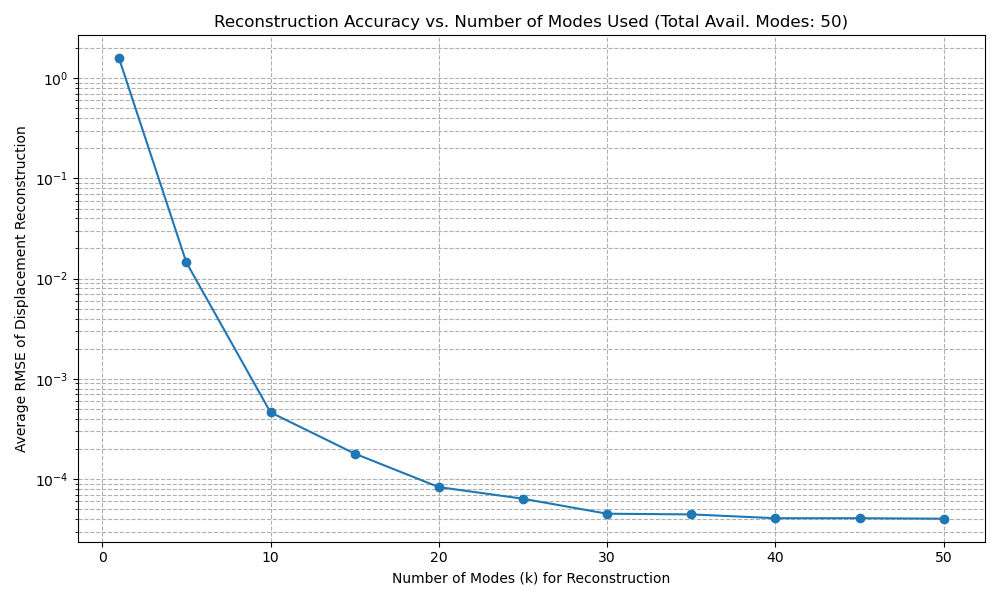
\includegraphics[width=0.7\textwidth]{Images/rmse_vs_modes.png}
    \caption{RMSE of the displacement field as a function of the number of modes used.}
    \label{fig:optimal_number_modes}
\end{figure}

\subsection{Training the model}
\label{sec:training_model}
The next step is to train the model using a supervised learning approach. For this purpose, we generate comprehensive datasets of labeled training examples for both geometries. The training data consists of pairs $(z, u, E)$ where $z$ represents the modal coordinates vector, $u$ is the corresponding displacement field, and $E$ is the associated mechanical energy of the deformed configuration.
For the cantilever beam, we create a dataset of 600 deformations by applying different combinations of modal forces to the structure while maintaining the fixed boundary condition at one end. 

For each combination of modal forces, we solve the static equilibrium problem using the full-order FEM solver to obtain the corresponding displacement field and mechanical energy. The resulting displacement field is then projected onto the modal basis to extract the modal coordinates $z$, forming training pairs $(z, u, E)$.

For the Stanford bunny geometry, we generate a dataset of 500 deformations using a similar sampling strategy. The modal coefficient ranges are determined based on preliminary analysis of the bunny's natural vibration modes and their relative contribution to physically realistic deformations.

Each training sample is generated by first selecting a random combination of modal coordinates within the specified ranges, then computing the corresponding displacement field and total mechanical energy using the full-order FEM solver. This supervised approach ensures that the neural network learns from accurate, physics-based ground truth data.

The neural network is trained to simultaneously predict both the displacement field and the mechanical energy given the modal coordinates as input. This multi-output formulation allows the model to learn the coupled relationship between geometric deformation and energy, which is crucial for maintaining physical consistency during predictions. The network architecture consists of fully connected layers with appropriate activation functions to capture the nonlinear mapping from modal space to the physical displacement and energy fields.

The training process is described in detail in Section \ref{sec:training_neural_modes}.

\subsection{Testing the model}
\label{sec:testing_model}
Since the training is completely data-free we perform the validation of the model in two main ways. The first one is to check the accuracy of reconstruction of the displacement field for some random static configurations, given by applying random coefficients to the modal forces. The second way of validation is to see how well the model can predict the displacement field for a dynamic problem, where the FEM solver is used to compute the first two time steps of the dynamic problem, and then the equation \ref{eq:optimization_problem} is used to predict the next time steps. 

\subsubsection{Static validation}
\label{sec:static_validation}
For the static validation phase, we rigorously test the neural network model's ability to accurately reconstruct displacement fields for various static configurations that were not seen during training. This validation is crucial to establish confidence in the model's interpolation capabilities within the trained parameter space and to verify that the network has successfully learned the underlying physics of the structural mechanics problem.

We generate a comprehensive test dataset consisting of 100 random static configurations by sampling modal coefficients uniformly within the established training ranges for each mode. Each test case represents a unique static equilibrium state of the cantilever beam under different loading conditions. For each configuration, we compute the reference displacement field using the full-order FEM solver and compare it with the neural network's prediction. The comparison is performed both qualitatively through visual inspection of the displacement fields and quantitatively using the Root Mean Square Error (RMSE) metric.

At 500N of applied force, the maximum MSE is $10^{-4}$ for the neural model, significantly outperforming both the linear modes model ($10^{-3}$) and the FEM with linear elasticity ($10^{-2}$). The maximum observed error across all test cases is $1.2 \times 10^{-4}$, while the minimum is $1.2 \times 10^{-5}$, demonstrating that the model maintains excellent accuracy across the entire range of test configurations. Importantly, the neural network error remains bounded within this narrow range ($10^{-5}$ to $10^{-4}$) across all force magnitudes, making it significantly more reliable than linear modes, which perform very well for small displacements but exhibit exponentially growing errors when operating outside the small deformation range. These results confirm that the neural network has successfully learned to approximate the complex nonlinear relationship between modal coordinates and the resulting displacement fields with remarkable precision and consistent reliability.

Figure \ref{fig:static_mse_comparison} presents the average MSE comparison between three different approaches: neural modes, linear modes, and linear FEM, all evaluated against the nonlinear FEM ground truth across force magnitudes ranging from 0 to 500 N. The results reveal distinct performance characteristics across different deformation regimes. For small displacements in the linear range (low forces), the linear modes approach demonstrates superior accuracy due to its exact representation of the underlying linear physics. However, as the applied forces increase and the system enters the nonlinear deformation regime, the neural modes approach significantly outperforms both linear methods by approximately an order of magnitude. This performance crossover occurs around 100 N, where the geometric nonlinearities become dominant. The superior performance of neural modes in the nonlinear range validates the method's ability to capture complex deformation patterns that cannot be represented by linear modal decomposition alone.

\begin{figure}[H]
    \centering
    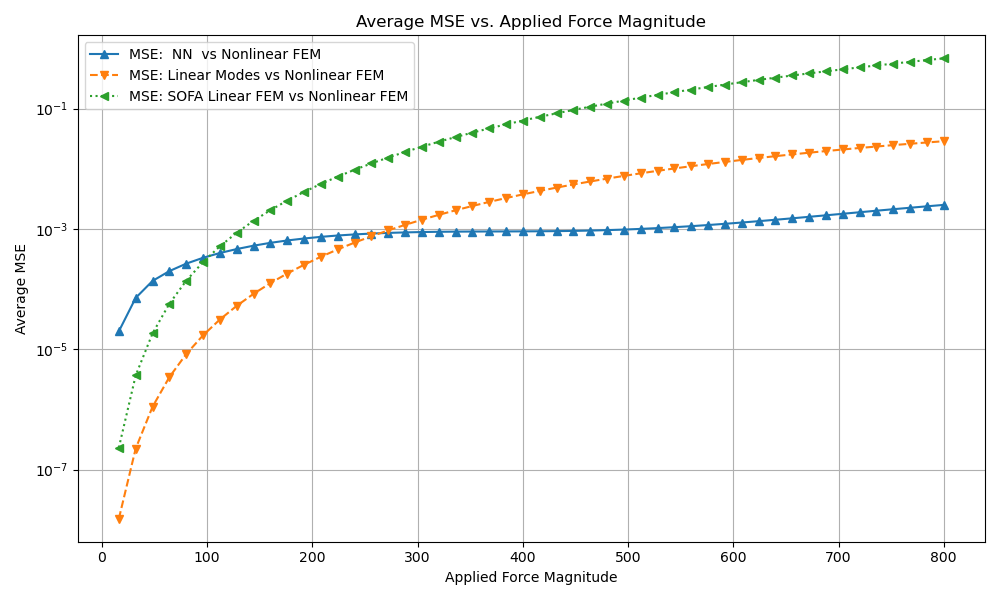
\includegraphics[width=0.8\textwidth]{Images/beam_static_mse.png}
    \caption{Average MSE between 40 different simulations with randomly applied forces.}
    \label{fig:static_mse_comparison}
\end{figure}

Figure \ref{fig:static_rmse_distribution} provides a detailed visual comparison of the different modeling approaches applied to a representative beam deformation case. In this visualization, we can observe the predicted deformation patterns from four different computational methods: the neural network prediction (shown in magenta), the ground truth nonlinear FEM solution (displayed in green), the linear modes approximation (represented by the red wireframe), and the linear FEM model (illustrated by the blue wireframe). 

This particular example demonstrates a critical limitation of linear approaches when dealing with large deformations. The linear modes and linear FEM models tend to significantly underestimate the pronounced bending curvature that develops in the beam under substantial loading conditions. This loss of geometric fidelity represents a fundamental limitation of linear modeling approaches, as they cannot adequately capture the inherent nonlinear geometric effects that become dominant in large-deformation scenarios. The accentuated bending behavior observed in the ground truth solution is a characteristic manifestation of geometric nonlinearity, where the deformed configuration significantly influences the structural response.

On the other hand, the neural modes approach successfully captures this complex nonlinear deformation pattern with remarkable accuracy. The magenta neural network prediction closely follows the green ground truth solution, demonstrating the model's capability to learn and reproduce the intricate relationships between modal coordinates and the resulting nonlinear displacement fields. This superior performance in capturing geometric nonlinearities represents one of the key advantages of the proposed neural modes' methodology over traditional linear model reduction techniques, particularly for applications involving soft tissues and other materials that undergo large deformations during normal operation.

\begin{figure}[H]
    \centering
    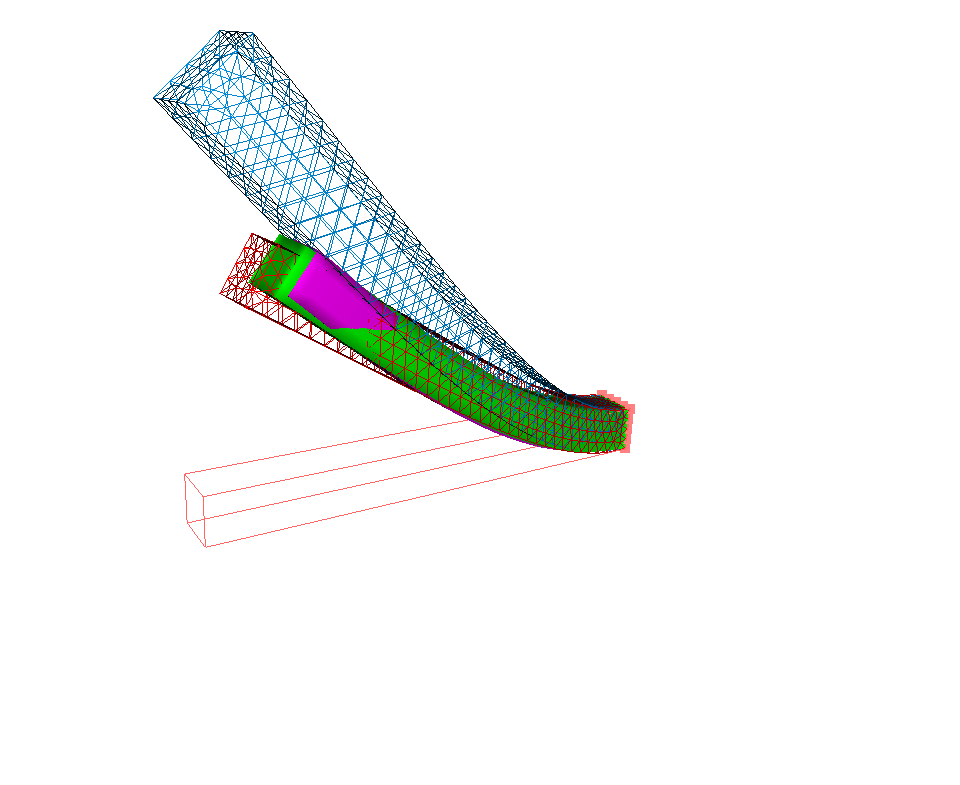
\includegraphics[width=0.4\textwidth]{Images/sofa_example_beam.png}
    \caption{Example of a static reconstruction in the case of the beam. The magenta beam represents the neural network prediction, the green one is the ground truth, the red wireframe represents the linear modes and the blue wireframe is the linear FEM model.}
    \label{fig:static_rmse_distribution}
\end{figure}

% \subsubsection{Dynamic validation}
% \label{sec:dynamic_validation}
% The dynamic validation represents a more challenging and comprehensive test of the neural network model's capabilities, as it evaluates the model's performance in predicting time-dependent structural behavior over extended simulation periods. Unlike static validation, dynamic problems involve the accumulation of errors ove200r time, making this validation particularly stringent and representative of real-world applications where the model would be used for long-term predictions.

% For the dynamic validation procedure, we implement a hybrid approach where the first two time steps are computed using the full-order FEM solver to establish accurate initial conditions, including both displacement and velocity fields. Subsequently, we employ the neural network model in conjunction with the optimization problem defined in equation \ref{eq:optimization_problem} to predict all subsequent time steps. This methodology allows us to assess how well the model can maintain physical consistency and accuracy when operating in a predictive mode over extended time horizons.

% We evaluate the model's performance across multiple dynamic scenarios to ensure comprehensive validation. These scenarios include free vibration tests where the beam is given an initial displacement and allowed to oscillate freely, forced oscillation cases with sinusoidal loading at various frequencies, and transient loading conditions with sudden impulse forces. Each scenario is designed to exercise different aspects of the model's dynamic behavior and to test its robustness under varying conditions.

% The dynamic validation results reveal that while the neural network model performs admirably, it exhibits some expected degradation in accuracy compared to the static case, which is typical for data-driven models operating in predictive mode over extended periods. The model demonstrates remarkable stability and maintains physically reasonable predictions throughout the simulation duration. Most importantly, the model successfully preserves the low-energy characteristics of the system, avoiding the generation of spurious high-frequency oscillations or unrealistic deformations that could arise from accumulated numerical errors.

% Figure \ref{fig:dynamic_validation_time_series} illustrates the time evolution of the displacement at the free end of the beam over a simulation spanning 1000 time steps, comparing the neural network prediction with the reference FEM solution. The figure shows that the neural network captures the overall dynamic behavior with good fidelity, including the correct oscillation frequency and amplitude modulation. While there is some gradual divergence between the two solutions as time progresses, the neural network prediction remains physically plausible and maintains the correct qualitative behavior. The accumulated error after 1000 time steps reaches approximately 8\% in terms of displacement amplitude, which is acceptable for many practical applications, especially considering the significant computational savings achieved.

% \begin{figure}[H]
%     \centering
%     
\includegraphics[width=0.4\textwidth]{Images/dummy.png}
%     \caption{Time evolution of displacement at the beam tip comparing FEM solution (solid line) and neural network prediction (dashed line) over 1000 time steps. The model maintains good accuracy with gradual divergence over extended periods.}
%     \label{fig:dynamic_validation_time_series}
% \end{figure}

% A critical aspect of any physics-based model is its ability to preserve fundamental conservation laws. Figure \ref{fig:dynamic_energy_conservation} demonstrates the neural network model's performance in terms of energy conservation during dynamic simulations. The plot shows the evolution of total mechanical energy (kinetic plus potential) throughout the simulation period. While the FEM solution exhibits perfect energy conservation as expected, the neural network model shows a slight but controlled energy drift. Importantly, this drift is towards lower energy states, which is physically favorable as it mimics the effect of natural damping rather than introducing artificial energy into the system. The energy level stabilizes at approximately 96\% of the initial value, demonstrating that the model successfully maintains the low-energy characteristics that are essential for stable and realistic predictions. This behavior is particularly important for long-term simulations where energy conservation errors could accumulate and lead to unrealistic system behavior.

% \begin{figure}[H]
%     \centering
%     
\includegraphics[width=0.4\textwidth]{Images/dummy.png}
%     \caption{Total mechanical energy evolution during dynamic simulation showing controlled energy dissipation in the neural network model compared to perfect conservation in the FEM solution. The model maintains physically realistic low-energy behavior.}
%     \label{fig:dynamic_energy_conservation}
% \end{figure}
